\section{Computer Vision}

The computer vision subsystem is a software component that is designed to recognise and track vehicles in images in order to count them and estimate their speed, henceforth to be referred to as the \emph{detection} component of the system. Each time an image is processed by the detection algorithm several subprocesses are performed in order to manipulate the original image into a state where vehicles have been isolated. These subprocesses can be seen in Figure \ref{fig:detection_design}. The vehicle tracking subprocess was largely influenced by the work of Adrian Rosebrock \cite{adrian_rosebrock_simple_object_tracking}\cite{adrian_rosebrock_vehicle_tracking} of PyImageSearch and the vehicle segmentation subprocess was influenced by the work of Andrey Nikishaev \cite{andrey_nikishaev_traffic_counting}. Much of the functionality is provided by the Python open source computer vision library, OpenCV \cite{opencv}


\begin{figure}[H]
    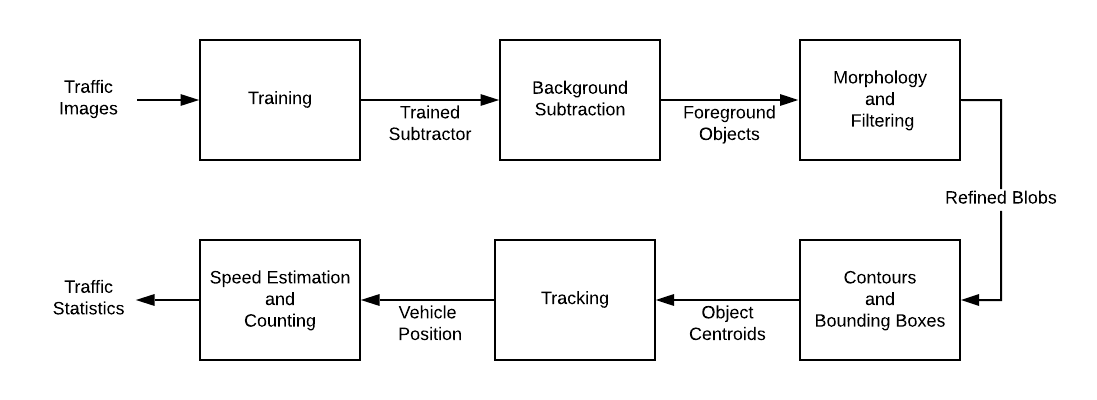
\includegraphics[width=0.9\columnwidth]{detection_design}
    \caption{Subprocess that comprise the detection subsystem.}
    \label{fig:detection_design}
\end{figure}


\subsection{The Background Subtractor}
\label{subsection:training}
The background subtractor is reposible for determining which pixels are background and which are foreground objects. The subtractor uses a Mixture of Gaussian model (section \ref{subsection:mog}) to cluster the pixels into those two sets - background and forground. Initially the model is 'trained' on several hundred images - a few seconds of video - so that it's immediate use yields the most accuracte statistics. The software implemntation of a Gaussian mixture model used is OpenCV's BackgroundSubtractorMOG2 function \cite{opencv_mog2}. This implementation is based on the research by Zoran Zivkovic and Ferdinand van der Heijden \cite{zivkovic_pattern_recognition} \cite{zivkovic_heijden_pattern_recognition_letters} in which a method of using a Gaussian Mixture Model (GMM) that improves upon former GMM in both speed and effectiveness at segmenting foreground objects, taking only a pixel's intensity as a feature. The subtraction component of the detection process was by far the most complex and thus the most computationally expensive, requiring each pixel in an image to have it's own probability density distrubtion and then to recalculate that for each new image. It was imperative, however, that the algorithm be fast enough that images could be processed as they arrived in real-time so that traffic data could reflect live conditions. Fortunately the speed of this implementation made it a suitable fit for a low power microcontroller and it's effectiveness ensured it's adoption into the system, as can be seen in Figure \ref{fig:example_subtraction}. This method is particularly effective at picking up moving objects as they cause pixels to have constantly changing intensities and making it easy for the model to determine that they're not a part of the background. 

Notice in Figure \ref{fig:foreground_mask_filtered} the gray pixels in and around the foreground objects, these are shadows that the OpenCV's GMM implemetation can explicitly detect. They are removed by thresholding (equation \ref{eq:threshold}) values that are not white and converting them to black (background) pixels.

\begin{figure*}[htbp]
    \centering 
    \begin{subfigure}[b]{0.45\textwidth}
        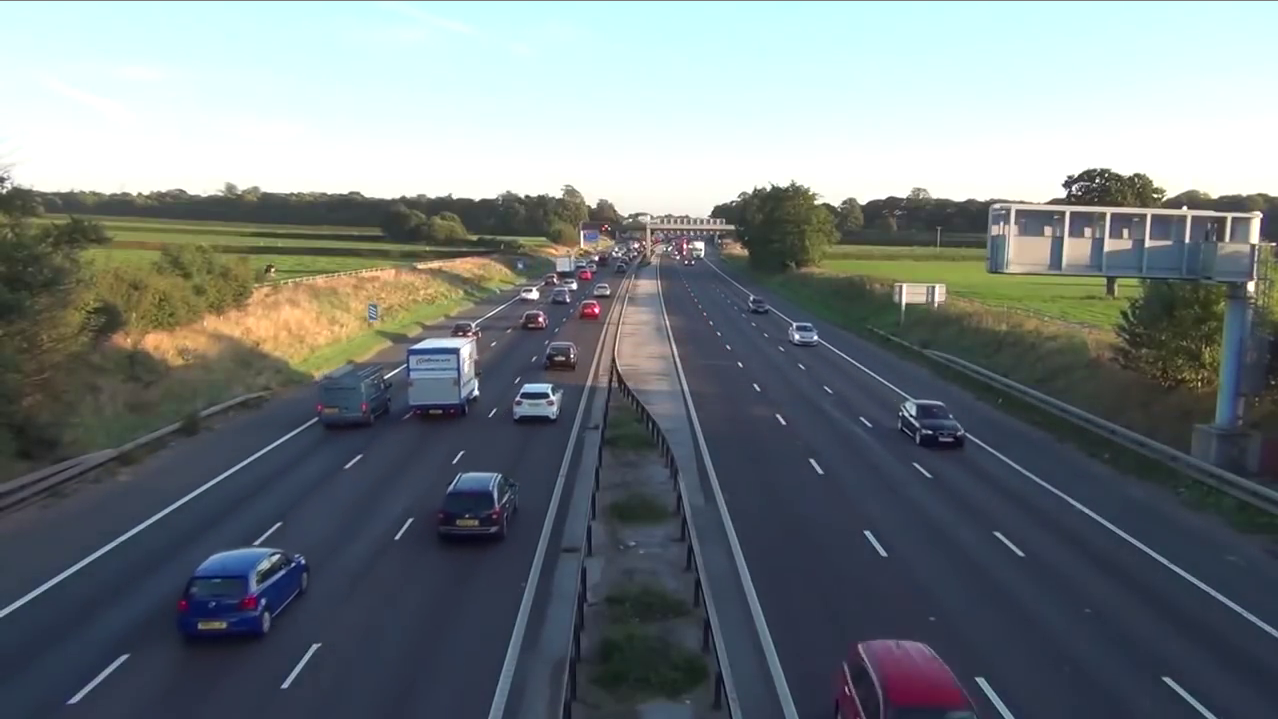
\includegraphics[width=\textwidth]{foreground_frame}
        \captionsetup{format = hang}
        \caption{The original frame of traffic. Img: Andrey Nikishaev.}
        \label{fig:frame_original}
    \end{subfigure}
    \begin{subfigure}[b]{0.45\textwidth}
        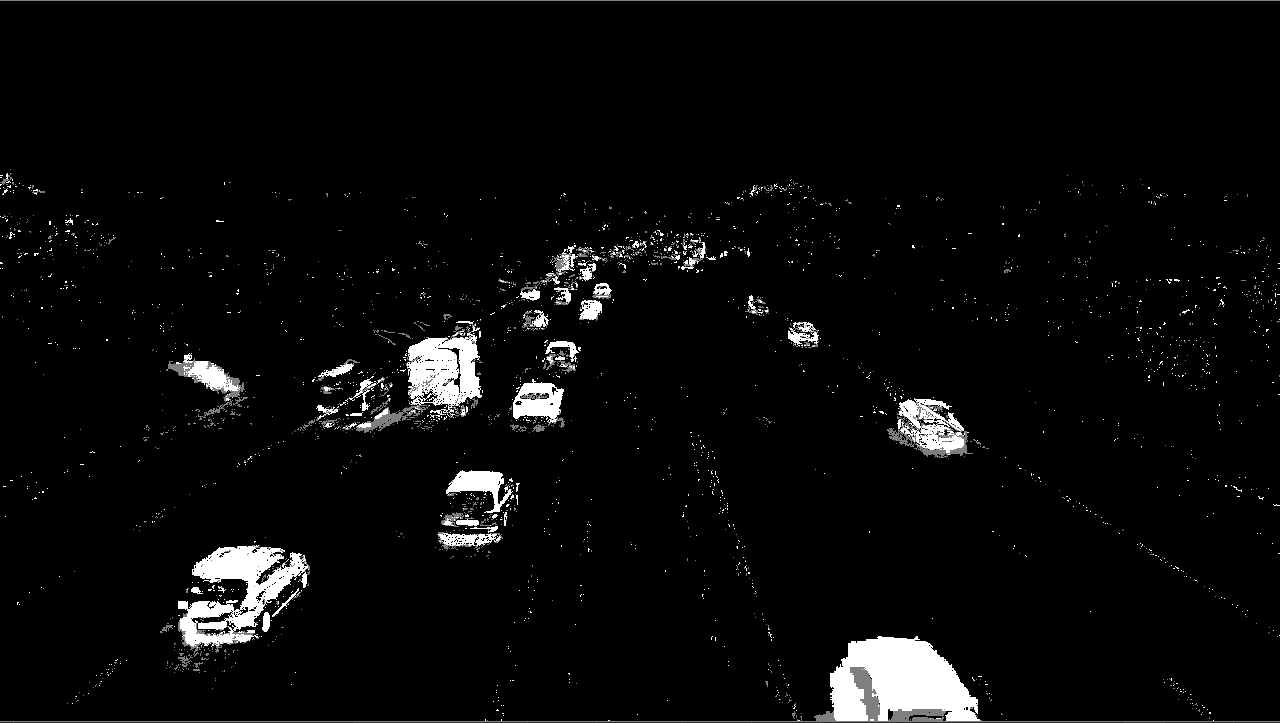
\includegraphics[width=\textwidth]{foreground_mask_unfiltered}
        \captionsetup{format = hang}
        \caption{Foreground mask generated by GMM clustering.}
        \label{fig:foreground_mask_unfiltered}
    \end{subfigure}
    \captionsetup{format=hang}
    \caption{A foreground mask generated from a traffic scene by OpenCV's GMM implementation.}
    \label{fig:example_subtraction}
\end{figure*}



\subsection{Morhpology and Filtering}

After isolating foreground objects it's necessary to remove noise and consolidate larger entities so that the only foreground pixels encountered by proceeding processes comprise vehicles. Because the GMM clusters pixels based on their value changes in lighting which might be caused by a cloud moving or a cars shadow among other others, can change the intensity of a background pixel and make it look like it's a foreground pixel. Furthermore, darker pixels, in car windows in particular, can make them appear like the road and hence background pixels, resulting in fractured foreground objects where only a single entitity should exist as in Figure \ref{fig:example_subtraction}.

\subsubsection{Filtering}

The noise generated by spurious foreground pixels looks a lot like salt and pepper noise and so to deal with this a median filter is applied to remove it (see Section \ref{subsection:median_filter}). The effect of this can be observed in Figure \ref{fig:foreground_mask_filtered}. It's important to remove this noise because it's evidently not a vehicle and will complicate proceeding image processing. 

\begin{figure*}[htbp]
    \centering 
    \begin{subfigure}[b]{0.45\textwidth}
        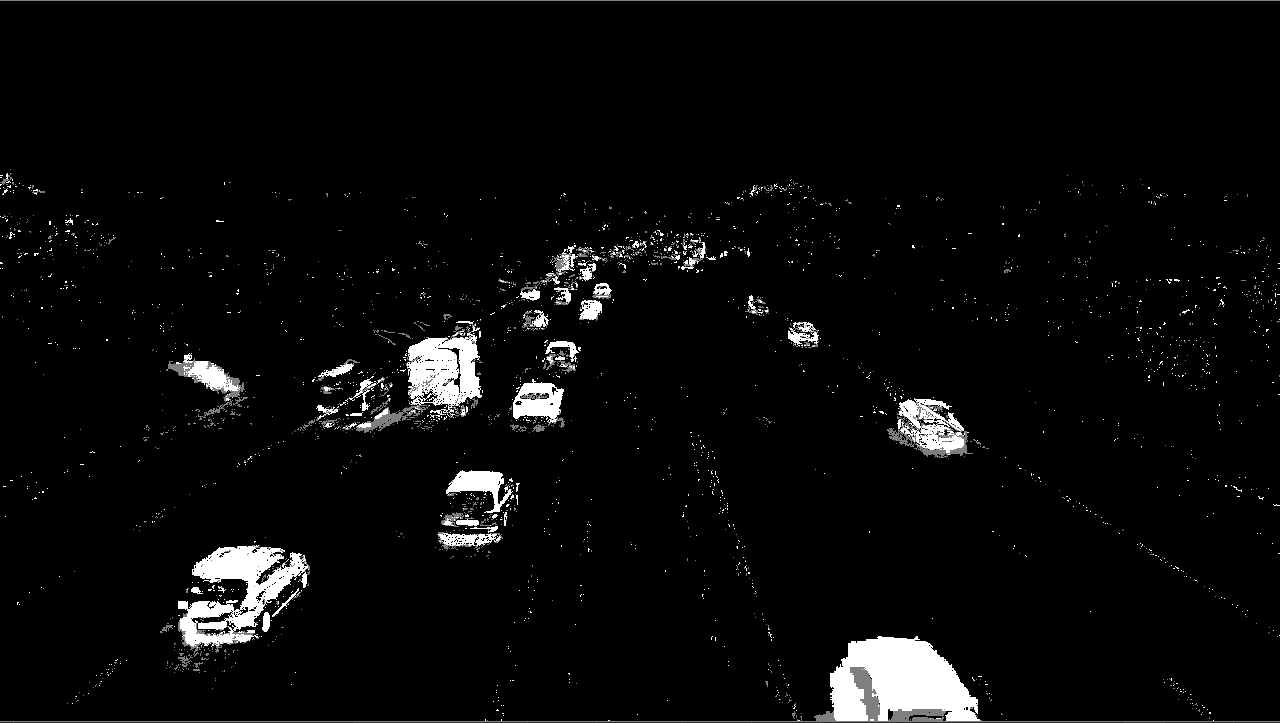
\includegraphics[width=\textwidth]{foreground_mask_unfiltered}
        \captionsetup{format = hang}
        \caption{Foreground mask generated by GMM clustering.}
    \end{subfigure}
    \begin{subfigure}[b]{0.45\textwidth}
        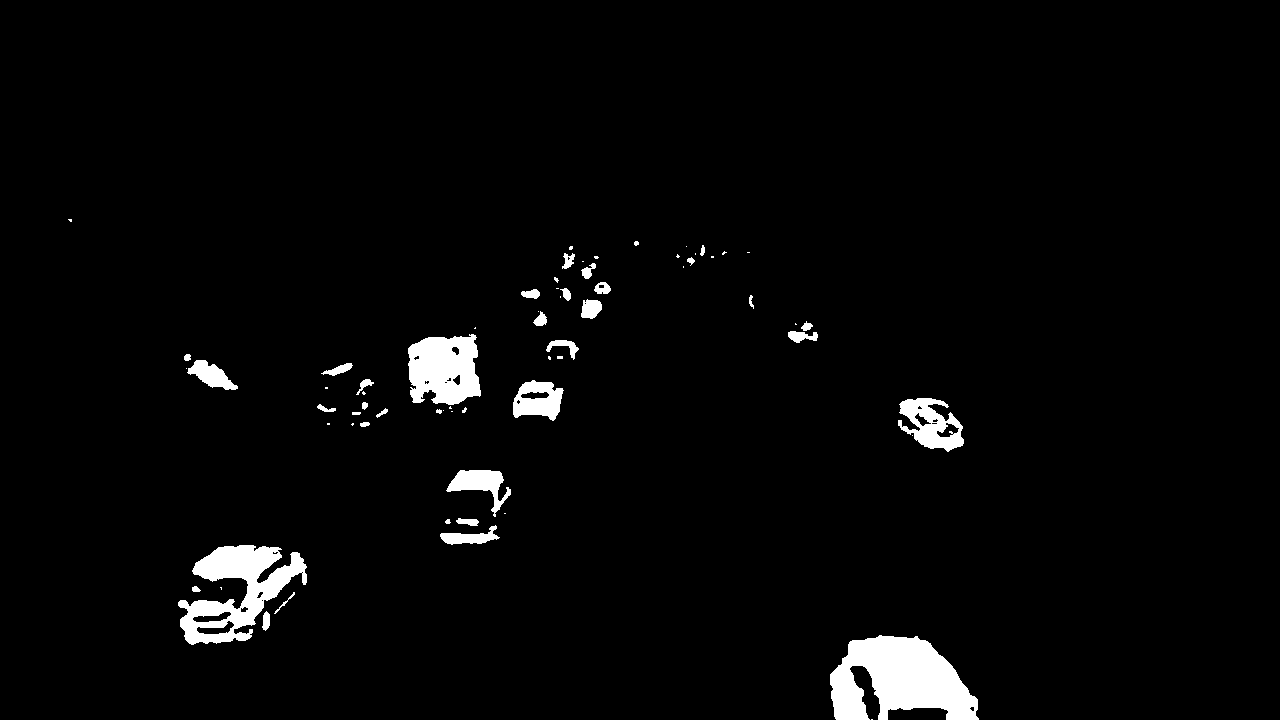
\includegraphics[width=\textwidth]{foreground_mask_filtered}
        \captionsetup{format = hang}
        \caption{Foreground mask denoised by 5x5 median filter.}
    \end{subfigure}
    \captionsetup{format=hang}
    \caption{A foreground mask generated from a traffic scene by OpenCV's GMM implementation.}
    \label{fig:foreground_mask_filtered}
\end{figure*}

\subsubsection{Morphology}

The foreground objects that are presented at this point are mostly correct and whole however some are fractured due to their windows reflecting the same color as the road. To consolidate these fractured entities an opening, closing and dilation (section \ref{section:morphology}) are performed, as can be seen in Figure \ref{fig:foreground_mask_morphed}. 

\begin{figure*}[htbp]
    \centering 
    \begin{subfigure}[b]{0.45\textwidth}
        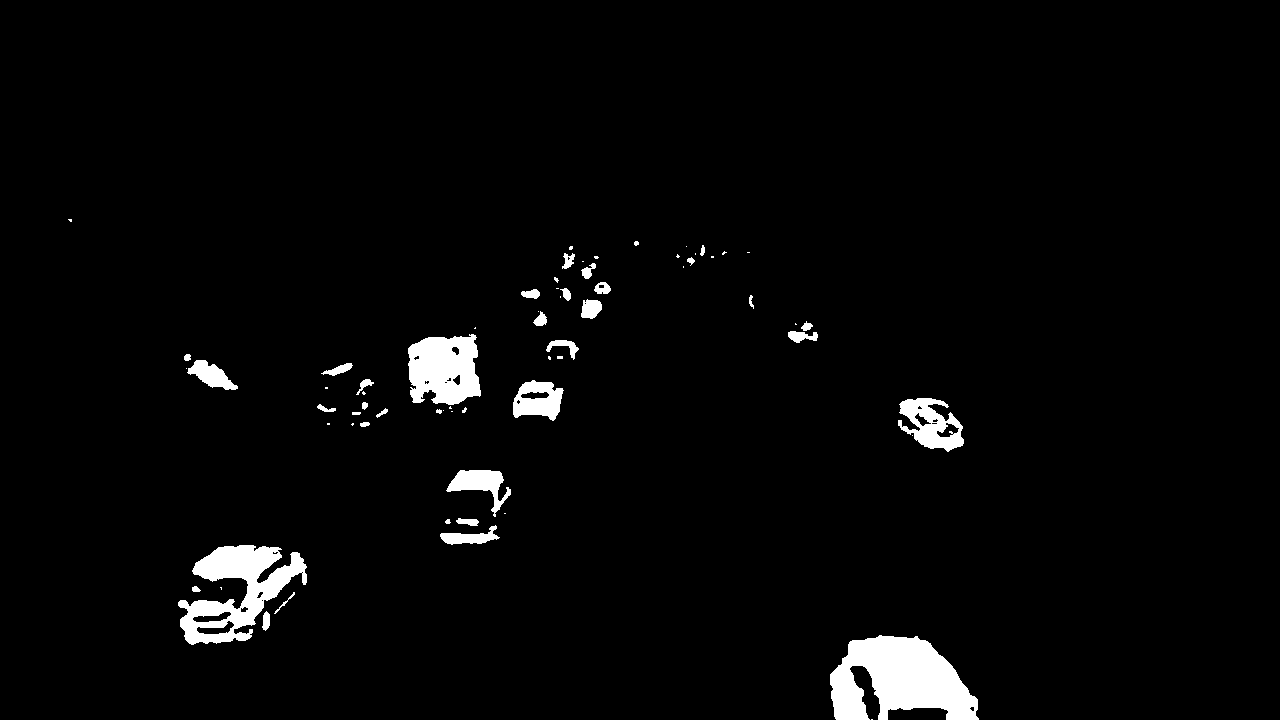
\includegraphics[width=\textwidth]{foreground_mask_filtered}
        \captionsetup{format = hang}
        \caption{Foreground mask denoised by 5x5 median filter.}
    \end{subfigure}
    \begin{subfigure}[b]{0.45\textwidth}
        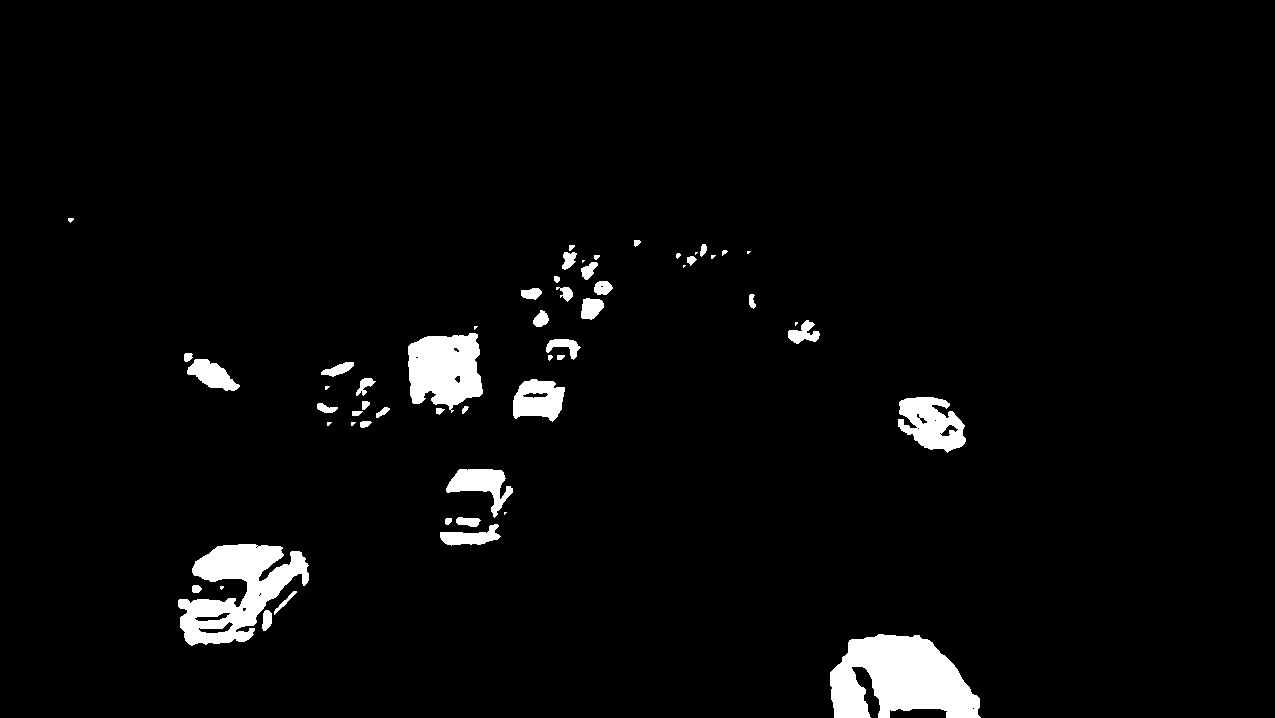
\includegraphics[width=\textwidth]{foreground_mask_morphed}
        \captionsetup{format = hang}
        \caption{Foreground mask closed, dilated.}
    \end{subfigure}
    \captionsetup{format=hang}
    \caption{A foreground mask generated from a traffic scene by OpenCV's GMM implementation.}
    \label{fig:foreground_mask_morphed}
\end{figure*}

In determining the calibration of each 

\subsection{Countours and Bounding Boxes}

Contours represent the outline of a foreground object and bounding boxes are the corrected squares that are placed around the polygons that represent an object's outline. These bounding boxes are important for in the tracking of a object.


\subsection{Tracking}

Tracking is follows an objects movement across multiple images. This requires that the object be reidentified in each new image and matched to it's old location.

\subsection{Speed Estimation and Counting}

This subprocess consolidates the efforts of the former ones and convert the information about an objects position into vehicle counts and speeds.

\subsection{Calibration}

It is unfortunate but neccessary that for this method of vehicle classification that for each different location and camera angle an element of calibration is required to obtain best results. This is a function of the size of vehicles in the camera frame and the lighting conditions at the location because the lighting alters what is perceived as a foreground object by the GMM and the size of the foreground objects is used to determine which objects are vehicles for given setting. Presently these factors are compensated for manually by calibration of the morphology and filtering subprocess. For example in finding the optimal morphological structuring element shape and size, and the number of iterations of closing and dilation to perform for the setting in Figure \ref{fig:original_frame} a visual analysis of the effect of a number of setting was performed as in Figure \ref{fig:morph_analysis}. This analysis must be performed for each node location where the desire is to achieve recognition of the most vehicles as foreground objects with the least fracturing and the diminishing of those objects that are not vehicles.

\begin{figure*}[htbp]
    \centering 
    \begin{subfigure}[b]{0.45\textwidth}
        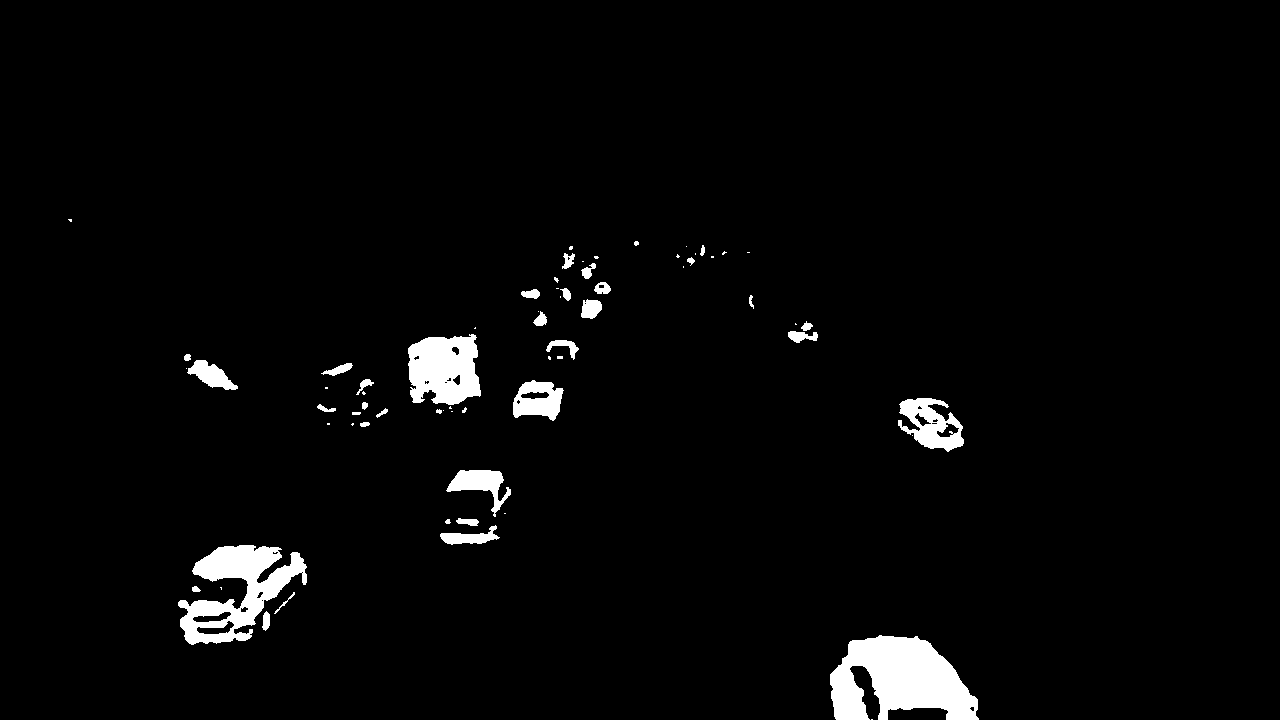
\includegraphics[width=\textwidth]{foreground_mask_filtered}
        \captionsetup{format = hang}
        \caption{Foreground mask denoised by 5x5 median filter.}
    \end{subfigure}
    \begin{subfigure}[b]{0.45\textwidth}
        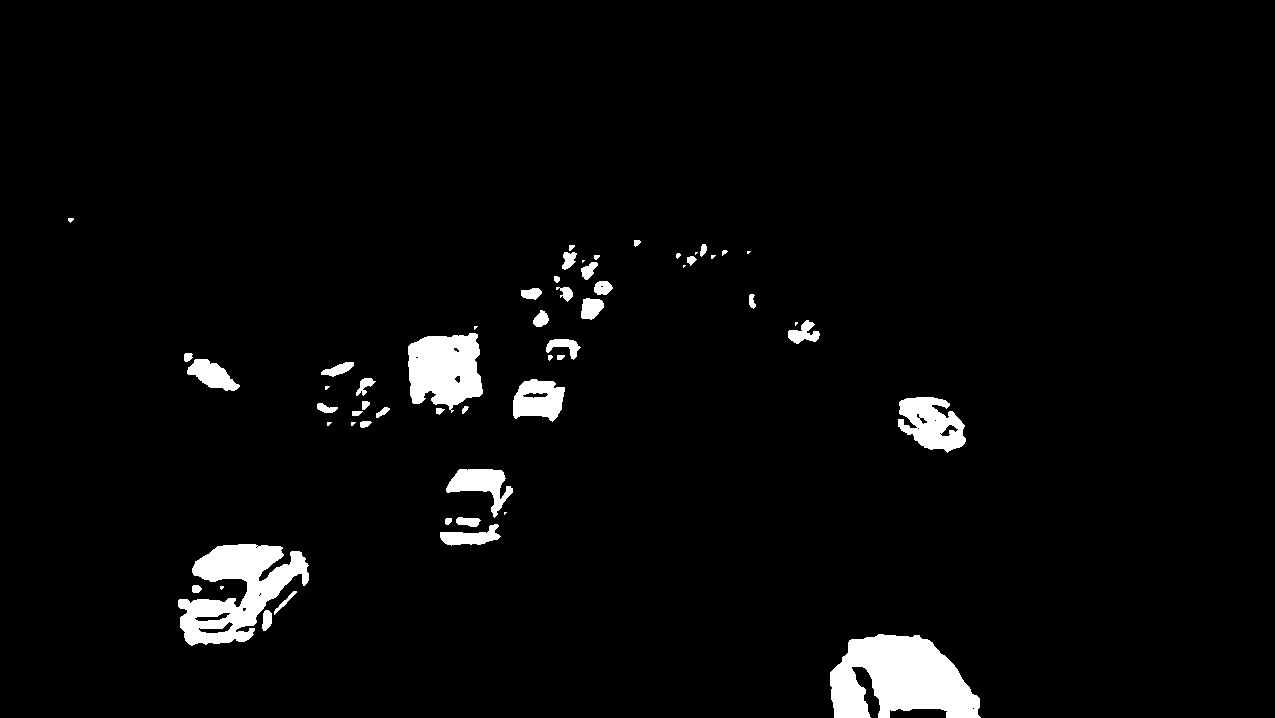
\includegraphics[width=\textwidth]{foreground_mask_morphed}
        \captionsetup{format = hang}
        \caption{Foreground mask closed, dilated.}
    \end{subfigure}
    \begin{subfigure}[b]{0.45\textwidth}
        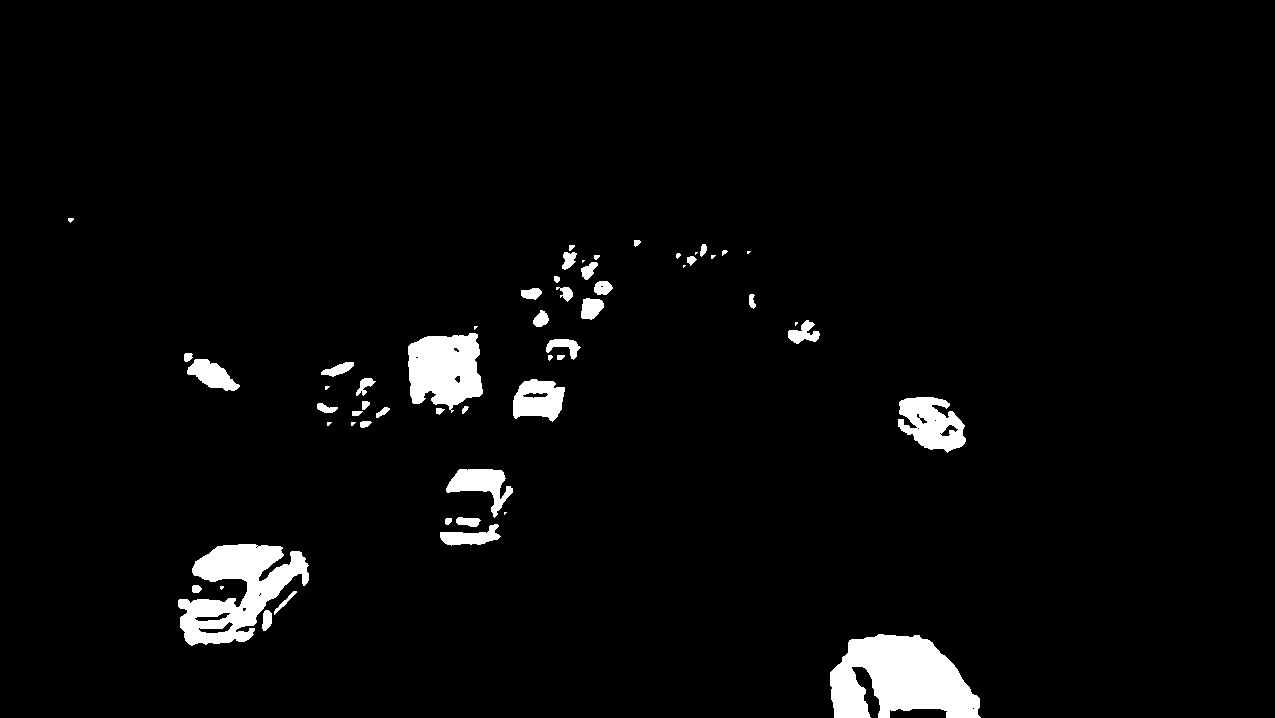
\includegraphics[width=\textwidth]{foreground_mask_morphed}
        \captionsetup{format = hang}
        \caption{Foreground mask closed, dilated.}
    \end{subfigure}
    \begin{subfigure}[b]{0.45\textwidth}
        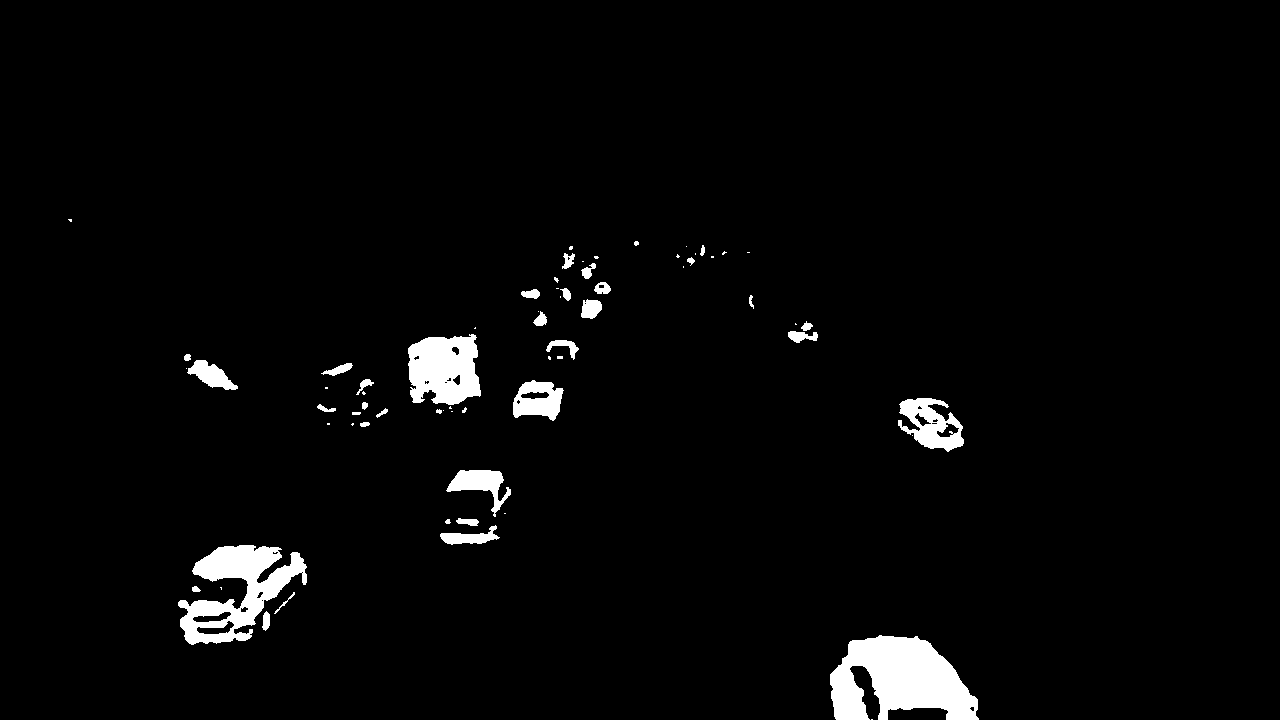
\includegraphics[width=\textwidth]{foreground_mask_filtered}
        \captionsetup{format = hang}
        \caption{Foreground mask denoised by 5x5 median filter.}
    \end{subfigure}
    \begin{subfigure}[b]{0.45\textwidth}
        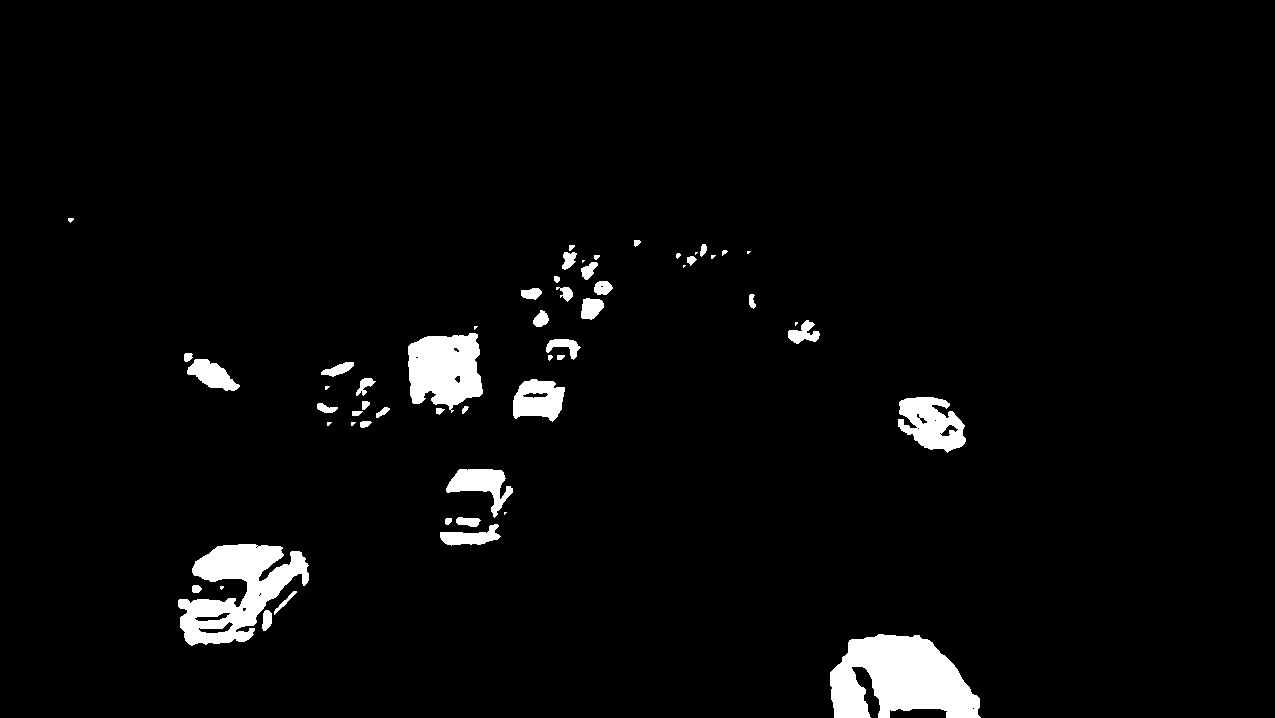
\includegraphics[width=\textwidth]{foreground_mask_morphed}
        \captionsetup{format = hang}
        \caption{Foreground mask closed, dilated.}
    \end{subfigure}
    \begin{subfigure}[b]{0.45\textwidth}
        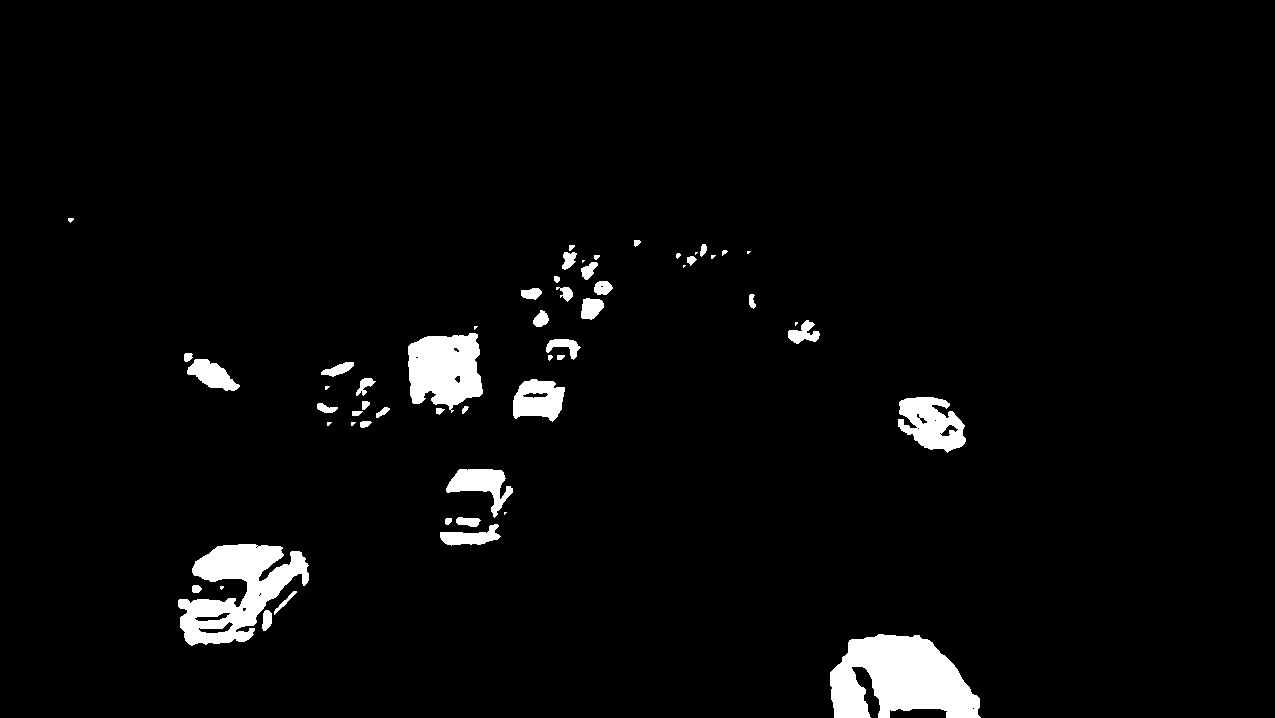
\includegraphics[width=\textwidth]{foreground_mask_morphed}
        \captionsetup{format = hang}
        \caption{Foreground mask closed, dilated.}
    \end{subfigure}
    \begin{subfigure}[b]{0.45\textwidth}
        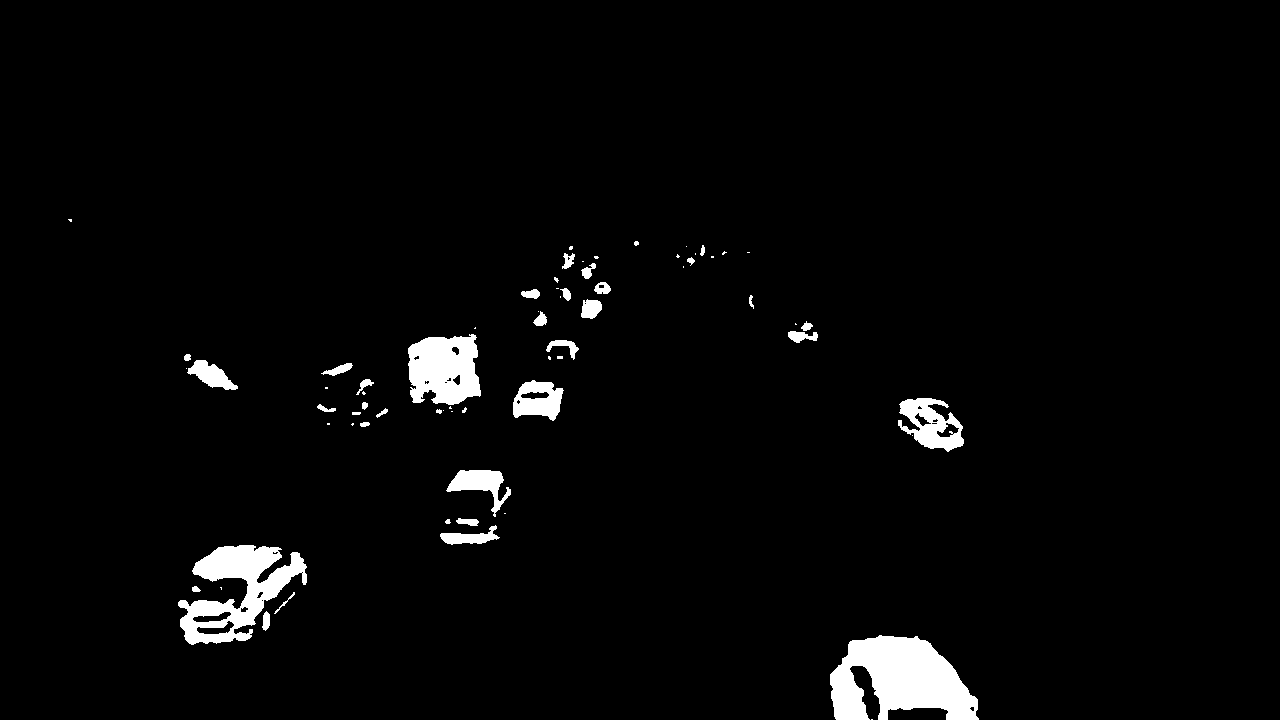
\includegraphics[width=\textwidth]{foreground_mask_filtered}
        \captionsetup{format = hang}
        \caption{Foreground mask denoised by 5x5 median filter.}
    \end{subfigure}
    \begin{subfigure}[b]{0.45\textwidth}
        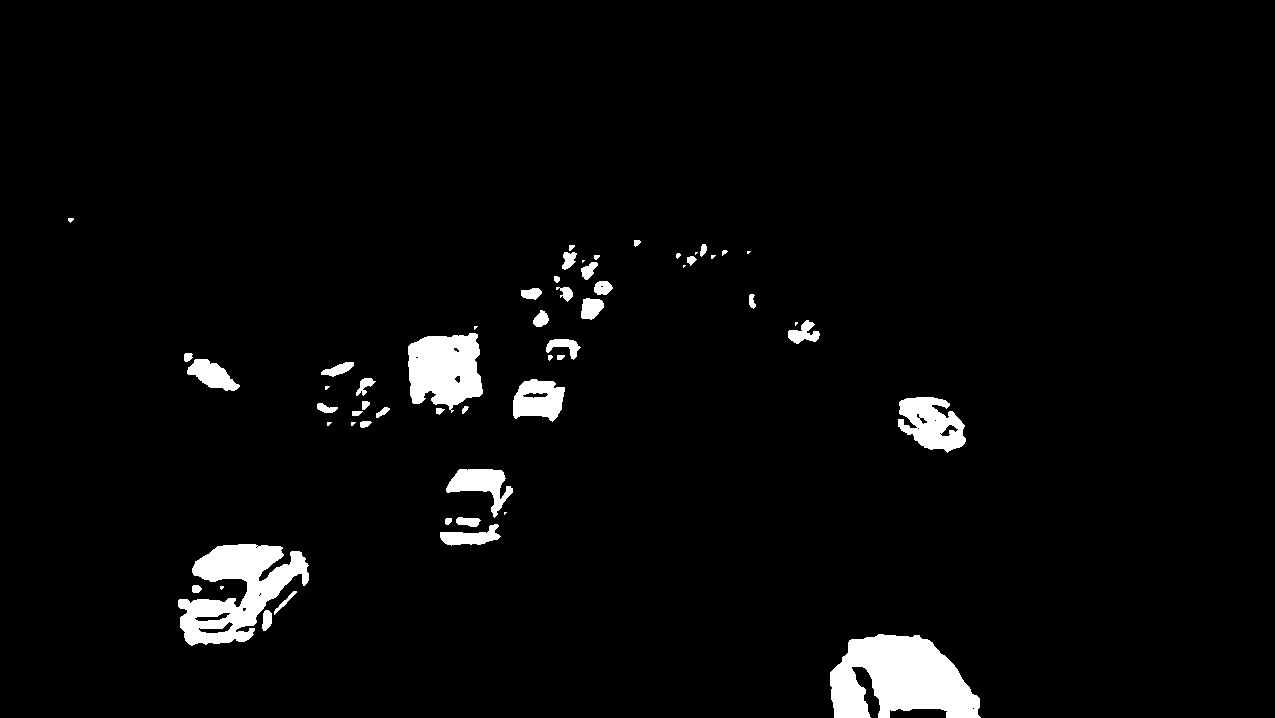
\includegraphics[width=\textwidth]{foreground_mask_morphed}
        \captionsetup{format = hang}
        \caption{Foreground mask closed, dilated.}
    \end{subfigure}
    \begin{subfigure}[b]{0.45\textwidth}
        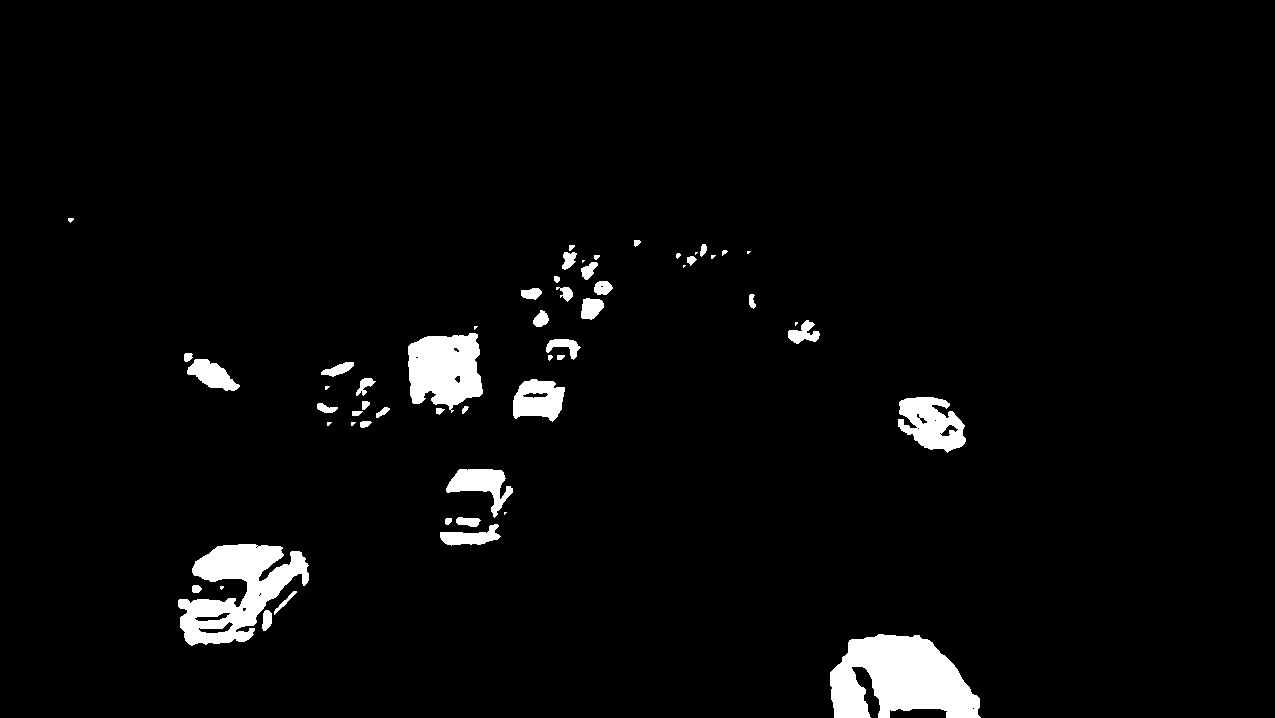
\includegraphics[width=\textwidth]{foreground_mask_morphed}
        \captionsetup{format = hang}
        \caption{Foreground mask closed, dilated.}
    \end{subfigure}
    \captionsetup{format=hang}
    \caption{A foreground mask generated from a traffic scene by OpenCV's GMM implementation.}
    \label{fig:foreground_mask_morphed}
\end{figure*}